\documentclass[conference]{IEEEtran}
\usepackage{cite}
\usepackage{amsmath,amssymb}
\usepackage{graphicx}
\usepackage{booktabs}
\usepackage{url}
\graphicspath{{../outputs/figures/}}

\begin{document}
\title{Predictive Maintenance of Turbofan Engines: Remaining Useful Life Prediction with Degradation Features and Classical Machine Learning (Phase 1)}
\author{\IEEEauthorblockN{Sarvesh Choudhary, Arun Jangir, Keshav Chhabra, Mayank Yadav, Rohit Kumar}
\IEEEauthorblockA{\textit{Advanced Machine Learning and Deep Learning Capstone, Project 7: Remaining Useful Life Prediction}\\
Code: \url{https://github.com/Arunjangir8/Capstone_AML}}}

\maketitle
\begin{abstract}
We predict the Remaining Useful Life (RUL) of turbofan engines on the NASA C-MAPSS FD001 subset as a supervised regression problem. Seven constant sensors are removed, the RUL target is capped at 125 cycles, and 71 features are built from past readings only: 10-cycle rolling mean, standard deviation and trend slope, and the deviation of each sensor from the engine's own healthy baseline. With a strict engine-level split (80 training, 20 validation engines) we compare Linear Regression, a Decision Tree and a Random Forest, tuned with grouped 3-fold cross-validation. On the official 100-engine test set the Random Forest is best, with RMSE 11.44 cycles, MAE 8.27 and $R^2$ 0.918, against 41.94 for a mean predictor. The engineered features cut the Random Forest's validation RMSE by 35.3\% compared with raw sensors, and baseline-deviation features carry 85.5\% of its importance.
\end{abstract}

\begin{IEEEkeywords}
Predictive maintenance, remaining useful life, C-MAPSS, feature engineering, random forest, decision tree
\end{IEEEkeywords}

\section{Introduction}
Turbofan engines wear gradually during operation. Estimating the Remaining Useful Life (RUL), the number of cycles left before failure, lets operators move from fixed-interval or reactive maintenance to condition-based maintenance: parts are replaced when they need to be, not too early and not too late.

Raw sensor readings are noisy and change slowly, so a single reading says little about health. In this first phase we test how far classical machine learning can go when it is given features that describe degradation explicitly. The contributions are: (1) a leakage-free pipeline with an engine-level split; (2) 71 degradation features computed from past readings only; (3) a tuned comparison of Linear Regression, a Decision Tree and a Random Forest on the official test set; and (4) an analysis of which features matter and where in engine life the errors occur. These results are the benchmark for Phase 2.


\section{Related Work}
Saxena \textit{et al.} \cite{r1} created the C-MAPSS run-to-failure simulation and its asymmetric scoring function. Data-driven prognostics commonly regresses RUL from window statistics of sensor signals using linear models and tree ensembles; Breiman's Random Forest \cite{r2} is a strong default for such tabular problems because averaging many decorrelated trees reduces variance. Later work moved to deep sequence models \cite{r3}, which we study in Phase 2.


\section{Dataset and Exploratory Analysis}
\subsection{C-MAPSS FD001}
FD001 simulates high-pressure compressor degradation under one operating condition. The training set has 100 engines run to failure (20,631 cycles); the test set has 100 engines whose records stop before failure, with the true RUL supplied separately. Each row has the engine id, the cycle, 3 operating settings and 21 sensors. There are no missing values or duplicate rows.

\subsection{Sensor Selection}
Seven sensors (s1, s5, s6, s10, s16, s18, s19) are constant or nearly constant and carry no information, and the operating settings are effectively fixed in FD001. We keep the 14 remaining sensors. The sensors most correlated with RUL are s11 (r = -0.70), s4 (-0.68), s12 (0.67) and s7 (0.66).

\subsection{Engine Lifetimes}
Training engines last between 128 and 362 cycles (mean 206, median 199). Fig. 1 shows that sensor values stay flat early in life and drift as failure approaches, which motivates both the capped target and the drift features below.

\begin{figure}[!t]
\centering
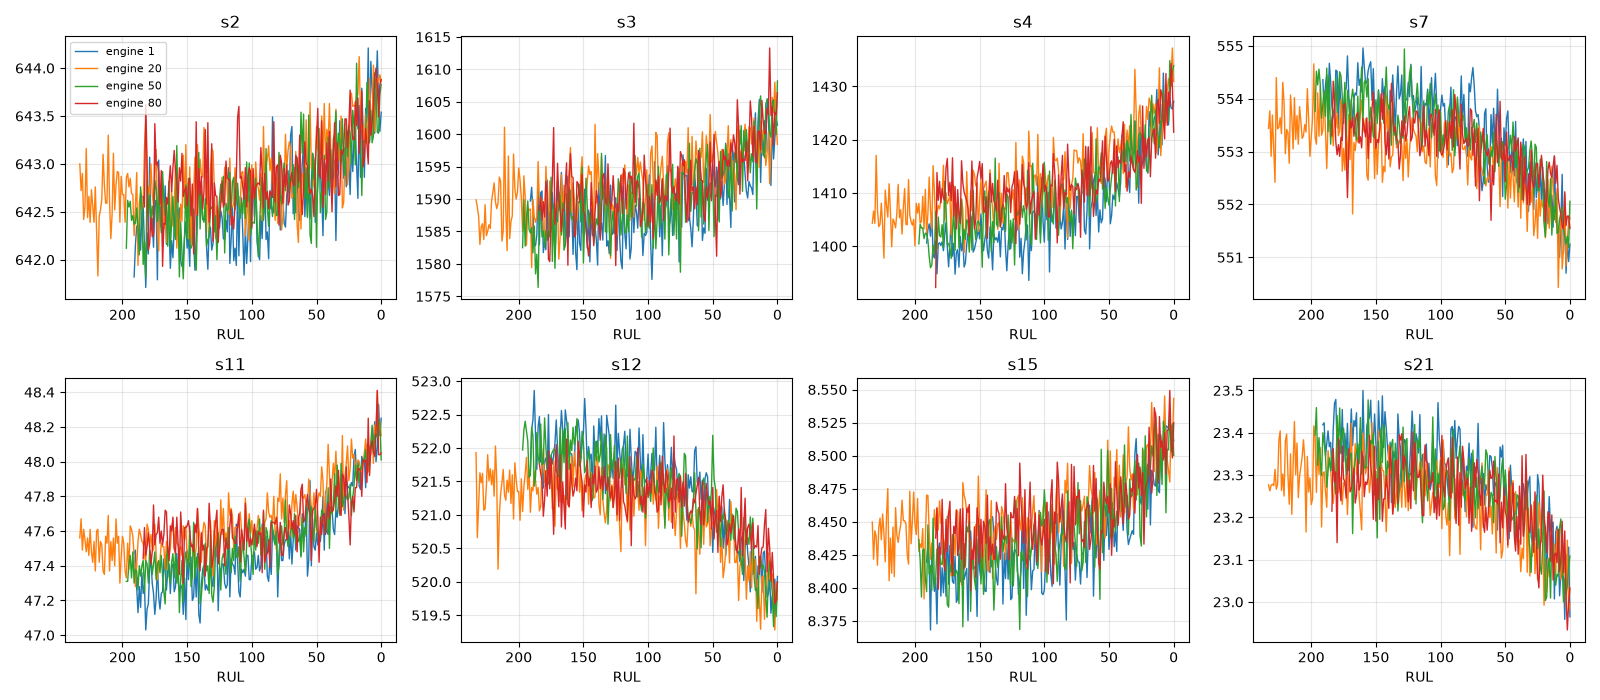
\includegraphics[width=\columnwidth]{01_sensor_trends.png}
\caption{Selected sensor readings over the life of several training engines. Degradation appears as a slow drift late in life.}
\label{fig1}
\end{figure}


\section{Methodology}
\subsection{Target}
Early in life the sensors cannot distinguish an engine with 300 cycles left from one with 200. We therefore use a piecewise-linear target capped at 125 cycles:

\begin{equation}
y_{i,t} = \min\left(125,\ T_i - t\right)
\label{eq1}
\end{equation}
where $T_i$ is the last cycle of engine i.

\subsection{Engine-Level Split}
The 100 training engines are split with GroupShuffleSplit (seed 42) into 80 training and 20 validation engines, so every row of an engine is on one side only. Hyper-parameters are tuned with 3-fold GroupKFold on the training engines, which keeps engines intact inside each fold. Automated checks confirm that no engine appears in two splits and that no feature uses future cycles.

\subsection{Feature Engineering}
For each of the 14 sensors s we compute four features over a backward window of the last 10 cycles of the same engine: the rolling mean, the rolling standard deviation, the least-squares trend slope, and the deviation from the healthy baseline,

\begin{equation}
\Delta s(t) = \mu_s(t) - \frac{1}{10}\sum_{\tau=1}^{10} s(\tau)
\label{eq2}
\end{equation}
where $\mu$s(t) is the rolling mean. The baseline is each engine's own first 10 cycles, so engine-to-engine manufacturing differences cancel out. With the cycle number and the 14 raw sensors this gives 1 + 14 + 14 $\times$ 4 = 71 features (Fig. 2).

\begin{figure}[!t]
\centering
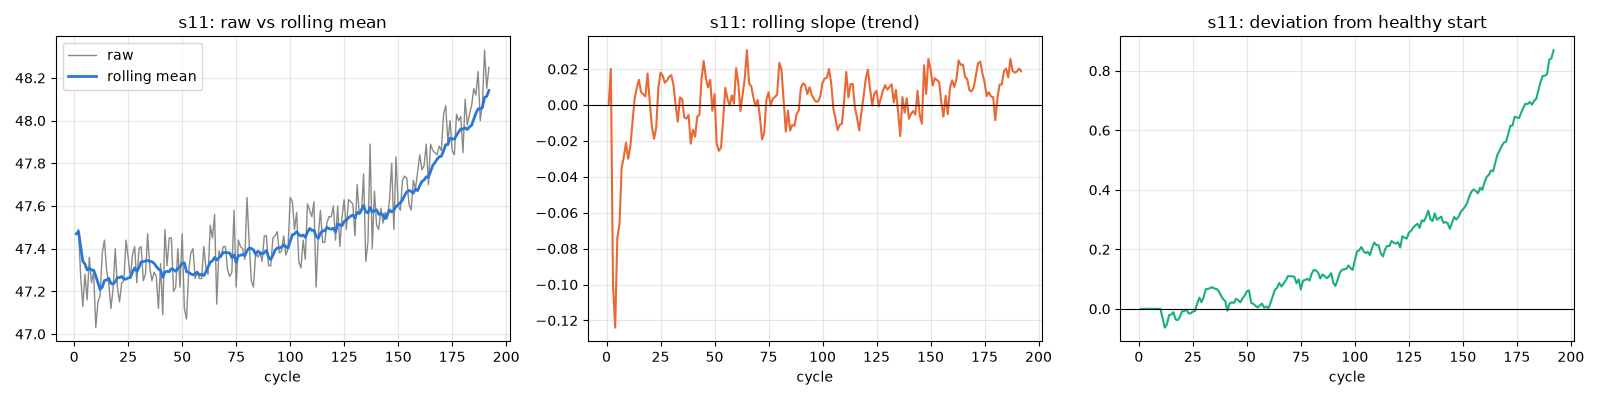
\includegraphics[width=\columnwidth]{02_features_example.png}
\caption{Raw sensor s11 of one engine with its rolling mean, slope and baseline-deviation features.}
\label{fig2}
\end{figure}

\subsection{Models}
\textbf{Linear Regression} (ordinary least squares on standardised features) is the simplest baseline and has no hyper-parameters. \textbf{Decision Tree} depth, minimum leaf size and cost-complexity pruning were searched over maximum depth in {5, 8, 12, none}, minimum leaf size in {1, 20, 50} and pruning strength $\alpha$ in {0, 1, 10}; the best setting is depth 12, leaf size 50, no pruning (CV RMSE 13.92). \textbf{Random Forest} uses 150 trees with all features considered at each split; the search over maximum depth in {10, 20} and minimum leaf size in {5, 20} selected depth 20 and leaf size 5 (CV RMSE 10.94). A mean predictor serves as the baseline every model must beat.

\subsection{Metrics}
We report RMSE, MAE and $R^2$ in cycles. Each test engine is scored once, at its last recorded cycle, against the capped true RUL.


\section{Results}
\subsection{Validation and Test Performance}
Table I shows that all three models beat the mean baseline by a wide margin and that the ranking on validation carries over to the test set. Linear Regression cannot follow the flat-then-falling shape of the target. The single tree fits it but is unstable; averaging 150 trees removes much of that variance, and the Random Forest is best on every metric.

\begin{table}[!t]
\caption{Validation (20 engines) and test (100 engines) RMSE, MAE and $R^2$}
\label{tabI}
\centering
\footnotesize
\begin{tabular}{lcccc}
\toprule
Model & Val RMSE & Test RMSE & Test MAE & Test $R^2$ \\
\midrule
Mean baseline & 41.72 & 41.94 & 34.83 & -0.095 \\
Linear Regression & 15.29 & 15.85 & 12.84 & 0.844 \\
Decision Tree & 14.13 & 14.96 & 10.80 & 0.861 \\
\textbf{Random Forest} & \textbf{10.34} & \textbf{11.44} & \textbf{8.27} & \textbf{0.918} \\
\bottomrule
\end{tabular}
\end{table}

\begin{figure}[!t]
\centering
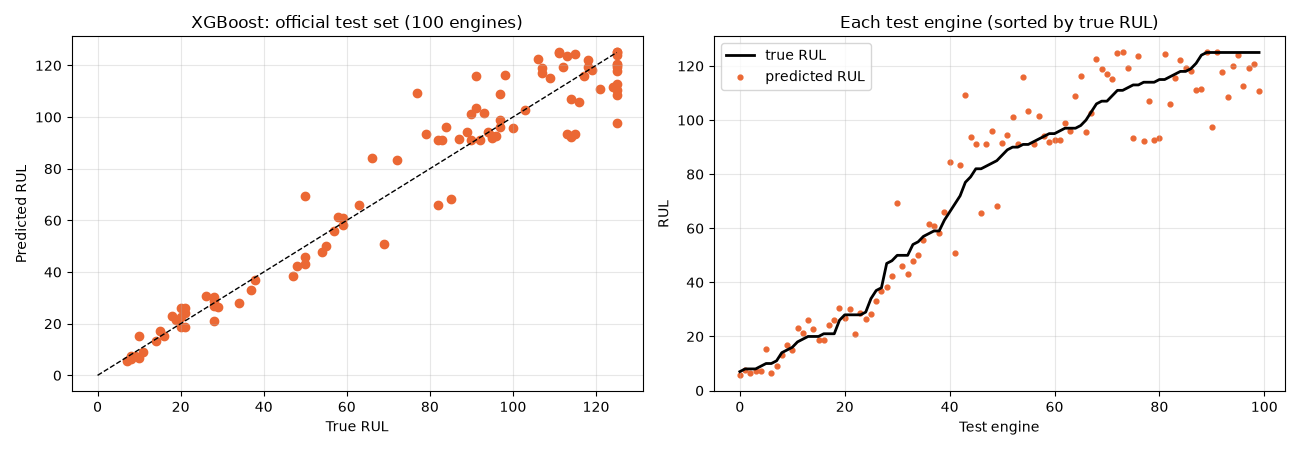
\includegraphics[width=\columnwidth]{06_best_model_test.png}
\caption{Random Forest predictions on the 100 official test engines.}
\label{fig3}
\end{figure}

\subsection{Effect of Feature Engineering}
To measure the value of the features we retrained each model on the 14 raw sensors plus the cycle number only (Table II). Every model improves, and the Random Forest gains the most because it can exploit the non-linear relation between drift and RUL.

\begin{table}[!t]
\caption{Validation RMSE with raw sensors versus engineered features}
\label{tabII}
\centering
\footnotesize
\begin{tabular}{lccc}
\toprule
Model & Raw (15) & Engineered (71) & Gain \\
\midrule
Linear Regression & 17.37 & 15.29 & 12.0\% \\
Decision Tree & 17.73 & 14.13 & 20.3\% \\
\textbf{Random Forest} & 15.98 & \textbf{10.34} & \textbf{35.3\%} \\
\bottomrule
\end{tabular}
\end{table}

\subsection{Feature Importance}
Grouping the Random Forest's impurity-based importances by feature type, baseline-deviation features account for 85.5\%, rolling means 11.0\%, the cycle number 2.4\%, and standard deviation, slope and raw sensors together about 1\%. A single feature, the drift of s11 (high-pressure compressor outlet static pressure) from its baseline, holds 74.0\% of the importance. How far an engine has moved from its own healthy state is far more informative than the absolute sensor value.

\subsection{Early versus Late Life}
Table III splits validation error by stage. All models are more accurate while the engine is healthy (RUL $>$ 100), where the target is flat at the cap, and less accurate in the late stage, where wear accelerates and differs between engines. The Random Forest has the lowest error in both stages.

\begin{table}[!t]
\caption{Validation RMSE by life stage}
\label{tabIII}
\centering
\footnotesize
\begin{tabular}{lcc}
\toprule
Model & Early ($>$100) & Late ($\le$100) \\
\midrule
Mean baseline & 35.67 & 47.07 \\
Linear Regression & 12.23 & 17.86 \\
Decision Tree & 10.01 & 17.33 \\
\textbf{Random Forest} & \textbf{8.01} & \textbf{12.26} \\
\bottomrule
\end{tabular}
\end{table}


\section{Limitations}
The study covers FD001 only, with a single operating condition and fault mode. Features use a fixed 10-cycle window that was not tuned. The late-stage error, which matters most for maintenance, is still about 50\% higher than the early-stage error, and summary features discard the order of readings inside the window. Phase 2 addresses this last point with sequence models.


\section{Conclusion}
Classical models with well-designed degradation features predict turbofan RUL accurately. The Random Forest reaches a test RMSE of 11.44 cycles, $R^2$ 0.918, and the features improve it by 35.3\% over raw sensors. The most useful signal is each sensor's drift from the engine's own healthy baseline. This result is the reference point for the deep learning models of Phase 2.


\begin{thebibliography}{00}
\bibitem{r1} A. Saxena, K. Goebel, D. Simon, and N. Eklund, ``Damage propagation modeling for aircraft engine run-to-failure simulation,'' in \textit{Proc. Int. Conf. Prognostics and Health Management}, 2008, pp. 1--9.
\bibitem{r2} L. Breiman, ``Random forests,'' \textit{Machine Learning}, vol. 45, no. 1, pp. 5--32, 2001.
\bibitem{r3} S. Zheng, K. Ristovski, A. Farahat, and C. Gupta, ``Long short-term memory network for remaining useful life estimation,'' in \textit{Proc. IEEE Int. Conf. Prognostics and Health Management}, 2017, pp. 88--95.
\end{thebibliography}

\end{document}
